\documentclass[18pt]{beamer}
\usepackage{tcolorbox}
\usepackage{templates/beamerthemekitwide}
\usepackage{ifthen}
\usepackage{pdfpages}
\usepackage{pifont}
\usepackage{hyperref}
\usepackage[autostyle]{csquotes}
\usepackage[hyperref,backend=biber,url=false]{biblatex}
\usepackage{pgfplots}
\pgfplotsset{compat=1.16}
\usepgfplotslibrary{statistics}
\usepackage{tikz}
\usetikzlibrary{decorations.pathreplacing,shapes,positioning}
\usepackage{siunitx}
\usepackage{marvosym}
\usepackage[clock]{ifsym}

\title[Analysis and Optimization of AVX DVFS]{Analysis and Optimization of Dynamic Voltage and Frequency Scaling for AVX Workloads Using a Software-Based Reimplementation}
\author{Yussuf Khalil}
\date{25 September 2019}
\institute{Operating Systems Group}
\titleimage{skylake_server_die_shot_intel_wikichip}

\addbibresource{presentation.bib}

\selectlanguage{english}

\definecolor{kitgreenexcl}{cmyk}{1.0,  0.0,  0.6, 0.0}
\definecolor{kitblue}     {cmyk}{0.8,  0.5,  0.0, 0.0}
\definecolor{kitgreen}    {cmyk}{0.6,  0.0,  1.0, 0.0}
\definecolor{kityellow}   {cmyk}{0.0,  0.05, 1.0, 0.0}
\definecolor{kitorange}   {cmyk}{0.0,  0.45, 1.0, 0.0}
\definecolor{kitbrown}    {cmyk}{0.35, 0.5,  1.0, 0.0}
\definecolor{kitred}      {cmyk}{0.25, 1.0,  1.0, 0.0}
\definecolor{kitpurple}   {cmyk}{0.25, 1.0,  0.0, 0.0}
\definecolor{kitcyan}     {cmyk}{0.9,  0.05, 0.0, 0.0}
\definecolor{kitgrey}	  {cmyk}{0.0,  0.0,  0.0, 0.15}
\definecolor{kitdarkgrey} {cmyk}{0.0,  0.0,  0.0, 0.5}

% https://tex.stackexchange.com/a/47797
\tikzset{ref/.style={insert path={%
			coordinate [pos=0,xshift=-0.5\pgflinewidth,yshift=-0.5\pgflinewidth] (#1 south west)
			coordinate [pos=1,xshift=0.5\pgflinewidth,yshift=0.5\pgflinewidth]   (#1 north east)
			coordinate [pos=.5] (#1 center)
			(#1 south west |- #1 north east)     coordinate (#1 north west)
			(#1 center     |- #1 north east)     coordinate (#1 north)
			(#1 center     |- #1 south west)     coordinate (#1 south)
			(#1 south west -| #1 north east)     coordinate (#1 south east)
			(#1 center     -| #1 south west)     coordinate (#1 west)
			(#1 center     -| #1 north east)     coordinate (#1 east)
}}}

\begin{document}
\selectlanguage{english}

\begin{frame}
	\titlepage
\end{frame}

\section{Motivation}
\begin{frame}[t]{Motivation}
	\begin{itemize}
		\item AVX is a modern vector processing extension for x86 processors
		\item Current Intel CPUs reduce their clock frequency when executing AVX code
		\item Lowered frequencies attained for a while after last AVX instruction
		\begin{itemize}
			\item[$\Rightarrow$] negative impact on performance in heterogeneous workloads
		\end{itemize}
	\end{itemize}
	\pause
	\begin{figure}
		\centering
		\vspace*{-0.7em}
		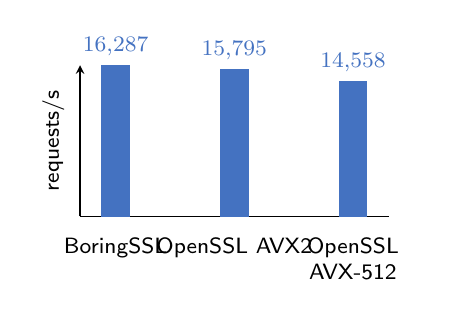
\begin{tikzpicture}[font=\footnotesize]
			\sffamily
			\begin{axis}[
				symbolic x coords={BoringSSL, OpenSSL AVX2, OpenSSL AVX-512},
				xtick=data,
				x tick label style  = {text width=2cm, align=center},
				ylabel={requests/s},
				axis y line=left,
				axis x line*=bottom,
				height=3.5cm,
				width=5.5cm,
				nodes near coords,
				ymin=0,
				ybar,
				enlarge x limits={0.15},
				ytick=\empty,
				xtick style={draw=none},
			]
			\addplot[fill=kitblue, color=kitblue] coordinates {
				(BoringSSL, 16287)
				(OpenSSL AVX2, 15795)
				(OpenSSL AVX-512, 14558)
			};
			\end{axis}
		\end{tikzpicture}
		\vspace*{-0.7em}
		\caption{nginx throughput with different ChaCha20-Poly1305 implementations\footfullcite{cloudflareinteldangers}}
	\end{figure}
\end{frame}

\section{Idea}
\begin{frame}[t]{Idea}
	\begin{itemize}
		\item Frequency switches are costly
		\begin{itemize}
			\item[$\Rightarrow$] wait before raising frequency after AVX execution
		\end{itemize}
		\pause
		\item What if we could predict when AVX code will be executed again?
		\item Could we raise the frequency earlier and improve performance during scalar phases?
	\end{itemize}
	\pause
	\begin{center}
		\vspace{1em}
		Try different reclocking algorithms!
	\end{center}
\end{frame}

\begin{frame}[t]{Idea}
	\begin{itemize}
		\item AVX reclocking is controlled solely by CPU itself
		\begin{itemize}
			\item We can not modify the hardware
			\begin{itemize}
				\item But we can (mostly) disable automatic reclocking
			\end{itemize}
			\item[$\Rightarrow$] reimplement algorithm in software
		\end{itemize}
		\pause
		\item Intel provides vague description of algorithm
		\begin{itemize}
			\item downclocking after $\leq$ \SI{500}{\micro\second}, upclocking after \SI{2}{\milli\second}, two frequency levels
			\item[$\Rightarrow$] need to analyze what the processors really do
		\end{itemize}
	\end{itemize}
\end{frame}
\chapter{Analysis}
\label{sec:analysis}

In order to be able to evaluate potential means of improving Intel's \gls{AVX} reclocking algorithm, we first need to obtain thorough knowledge of the algorithm as it is implemented in current Intel x86 \glspl{CPU}. We can then use this knowledge for the software-based reimplementation presented in \Cref{sec:design} and to understand the hardware-induced constraints Intel needs to keep within, which is in turn necessary for designing a feasible and implementable improved reclocking algorithm.

Intel regularly publishes optimization manuals~\cite{inteloptimizationmanual} intended for compiler developers and software engineers which contain a vague description of the mechanism used for deciding when to lower or raise the processor's frequency upon execution of \gls{AVX} instructions. Precisely, Intel defines three \textit{turbo license levels}, which designate frequency offsets for different instruction mix scenarios:

\begin{itemize}
	\item Level~0: only non-demanding (i.e., scalar, \gls{SSE}, \gls{AVX1} or light \gls{AVX2}) instructions are being executed; a core may run at its maximum turbo frequency. This is the default state.
	\item Level~1: active during the execution of heavy \gls{AVX2} and/or light \gls{AVX-512} instructions. The maximum frequency is lowered to a \gls{SKU}-specific value.
	\item Level~2: used for the execution of heavy \gls{AVX-512} instructions. The maximum frequency is lowered to a \gls{SKU}-specific value that is further below the frequency used in level~1.
\end{itemize}

Here, \enquote{heavy} instructions are defined to be floating-point, integer multiplication or integer \gls{FMA} operations. Given these license levels, Intel states that it may take up to \SI{500}{\micro\second} until the new frequency is applied and about \SI{2}{\milli\second} until a core reverts to level~0 after executing the last \enquote{heavy} instruction. Before the frequency is lowered, a core operates at \enquote{a lower peak capability}, however, Intel does not further specify what that exactly means. Intel hints that the license decisions are not solely bound to the instruction types as given in the level descriptions, but rather depend on the mix of instructions executed within a certain time window.

In this chapter we will describe the design of a framework that allows us to analyze the actual behavior of an x86 processor during the execution of \gls{AVX} instructions. Afterwards, we will present and evaluate the results generated when executed on a system equipped with a modern Intel \gls{CPU}. Finally, we compare our findings to what Intel maintains in their specification and point out deviations of the timings between the actual behavior and their claims.

\section{Methodology}
\label{sec:analysis:methodology}

For our reimplementation, our goal is to create a model of the reclocking behavior of an \gls{AVX-512}-capable \gls{CPU} that is as complete as possible and reflects the decisions made by the hardware with high accuracy. Therefore, by conducting this analysis, we want to answer the following aspects:

\begin{itemize}
	\item When exactly does a \gls{CPU} core decide to reduce or raise it's frequency during and after \gls{AVX} execution?
	\item How much time do turbo license level switches need?
	\item Do the \glspl{CPU} switch directly from level 0 to level 2 in case of heavy \gls{AVX-512} instructions or is there a step to level 1 in between?
	\item What does Intel mean by \enquote{lower peak capability} while lowering the clock?
	\item How complete is Intel's description of the reclocking algorithm?
\end{itemize}

In order to create a precise model we want to analyze these questions in different scenarios, i.e., for different instruction types, for different global load situations as well as with and without enabled turbo frequencies. To reach our goal, we run our analysis framework with synthetic code snippets that are designed to trigger the behavior to be analyzed.

\section{Design}
\label{sec:analysis:design}

Our analysis framework consists of a module for the Linux kernel as well as a user-space component which interact with each other and make use of the \gls{PMU}, a unit commonly found in modern microprocessors that enables software to measure performance and bottlenecks on the hardware level. In the following sections, we will present the design and features of these components and describe how they contribute to our analysis purposes.

\subsection{Performance Monitoring Unit (PMU)}
\label{sec:analysis:design:pmu}
Modern x86 \glspl{CPU} commonly feature a \gls{PMU} \cite{intelsdmsysprogguide} which exposes a set of \textit{performance counters} that may be configured to count assertions of a large set of \textit{performance events}.

Precisely, we use version~3 of the x86 \textit{Architectural Performance Monitoring} facility, which features three \textit{fixed counters} per logical core that count retired instructions, cycles during which the core is not in a halt state and \glsunset{TSC}\gls{TSC} cycles in unhalted state, respectively. The \glsreset{TSC}\gls{TSC} is a simple counter found in current x86 \glspl{CPU} that increments steadily with a fixed frequency, independent of the core clock, thus making it suitable for measuring wall-clock time. In addition to the fixed counters, eight freely configurable counters are available per physical core (four per logical core when \gls{SMT} is enabled). These counters may be set to count any of the performance events available for a specific microarchitecture, e.g., most architectures define events for cache hits/misses, execution stalls or load on specific execution units.

Each counter is represented via a \gls{MSR} and also configured through one. More specifically, software may configure the event to count (non-fixed counters only) and when to count (e.g., in user mode (ring~$\geq$~1) and/or kernel mode (ring~0)). Additionally, the counter can be configured to trigger an interrupt when it overflows. By setting the counter to its maximum value less an offset, this can be used as a mechanism to generate notifications when a certain amount of events of a specific type has occurred. The interrupt vector used for delivery can be configured in the core's \gls{APIC}'s \gls{LVT}. Optionally, the \gls{PMU} may be instructed to freeze all counters at their current values as soon as an interrupt is triggered.

\subsection{Overview}
\label{sec:analysis:design:overview}

The analysis tool presented here is made up of a kernel and a user-space component where the former provides the latter with means to configure the \gls{PMU} and efficient handling for interrupts generated by performance counter overflows.

As depicted in a simplified way in \Cref{fig:analysis:design:overview}, upon execution, the user-space component generates a \gls{PMU} configuration designed to produce the desired measurements, which is then applied by the kernel module. Now, the kernel module jumps back into user-space to an address previously defined by the user-space component which in turn executes \gls{AVX} instructions until preempted by an overflow interrupt generated by the \gls{PMU} according to its configuration (as described in \Cref{sec:analysis:design:pmu}).

\begin{figure*}
	\centering
	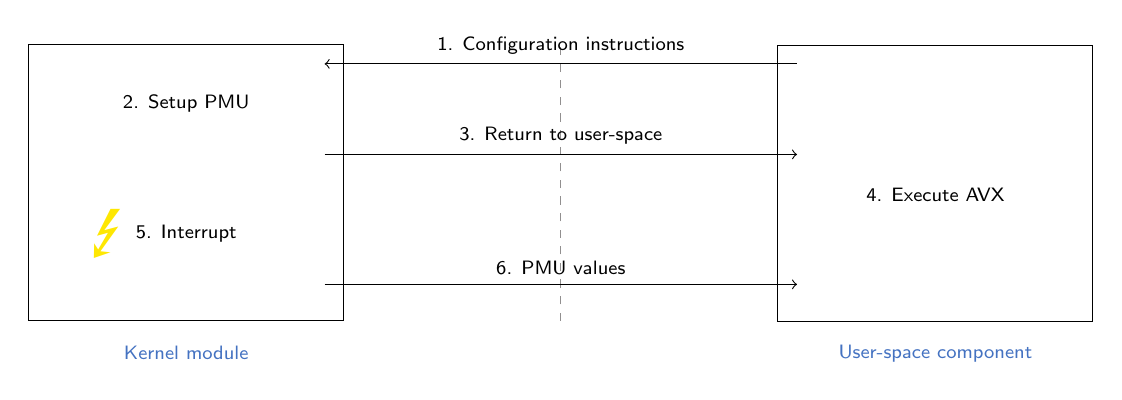
\begin{tikzpicture}[font=\scriptsize]
		\sffamily
		\pgfmathsetmacro{\componentrectwidth}{4}
		\pgfmathsetmacro{\componentrectheight}{3.5}
		\pgfmathsetmacro{\separatordist}{2.75}
		\pgfmathsetmacro{\arrowoverlength}{0.25}
		\pgfmathsetmacro{\arrowlength}{2*(\arrowoverlength + \separatordist)}

		% kernel
		\draw (0cm,0cm) rectangle ++(\componentrectwidth cm,\componentrectheight) [ref=kernel-rect];
		\node[color=kitblue] at ([yshift=-0.4 cm] kernel-rect south) {Kernel module};
		%\draw[densely dotted] ([yshift=-1cm] kernel-rect north west) -- ++(\componentrectwidth,0) [ref=kernel-sep];
		%\node at ([yshift=-0.5cm] kernel-rect north) {Linux};

		% separator
		\draw[dashed, color=kitdarkgrey] ([xshift=\separatordist cm] kernel-rect south east) -- ([xshift=\separatordist cm] kernel-rect north east) [ref=separator];

		% user-space
		\draw ([xshift=\separatordist cm] separator south east) rectangle ++(\componentrectwidth,\componentrectheight) [ref=user-rect];
		\node[color=kitblue] at ([yshift=-0.4 cm] user-rect south) {User-space component};

		% steps
		\draw[<-] ([yshift=-0.25cm,xshift=-\arrowoverlength cm] kernel-rect north east) -- ++(\arrowlength,0) node[align=center,pos=.5,above=0] {1. Configuration instructions};
		\node at ([yshift=-0.75cm] kernel-rect north) {2. Setup PMU};
		\draw[->] ([yshift=-1.4cm,xshift=-\arrowoverlength cm] kernel-rect north east) -- ++(\arrowlength,0) node[align=center,pos=.5,above=0] {3. Return to user-space};
		\node at ([yshift=-1.9cm] user-rect north) {4. Execute AVX};
		\node[color=kityellow] at ([yshift=-2.42cm,xshift=-1cm] kernel-rect north) {\Huge\Lightning};
		\node at ([yshift=-2.4cm] kernel-rect north) {5. Interrupt};
		\draw[->] ([yshift=-3.05cm,xshift=-\arrowoverlength cm] kernel-rect north east) -- ++(\arrowlength,0) node[align=center,pos=.5,above=0] {6. PMU values};
	\end{tikzpicture}
	\caption{Simplified analysis framework architecture. The kernel module enables the user-space component to configure the PMU and handles interrupts.}
	\label{fig:analysis:design:overview}
\end{figure*}

\subsection{Kernel Component}
\label{sec:analysis:design:kernel}

\subsection{User-Space Component}
\label{sec:analysis:design:userspace}

\subsection{Execution Modes}
\label{sec:analysis:design:executionmodes}
\section{Reimplementation}
\begin{frame}[t]{Design}
	\begin{itemize}
		\item Modify \texttt{intel\_pstate} Linux driver
		\begin{itemize}
			\item \texttt{intel\_pstate} manages core frequency
		\end{itemize}
		\item Introduce virtual AVX frequency levels similar to hardware levels
		\item Use performance counters to measure executed AVX instructions
		\begin{itemize}
			\item \textbf{Only available for floating-point}
		\end{itemize}
	\end{itemize}
\end{frame}

\begin{frame}[t]{Algorithm}
	\vspace*{-1em}
	\begin{enumerate}
		\item Interrupt after first 512-bit instruction
		\item Switch to level 1 frequency
		\item Measure instruction throughput in \SI{100}{\micro\second} intervals
		\item If higher than one per cycle: switch to level 2
		\item Raise frequency after \SI{666}{\micro\second} with no 512-bit instructions
	\end{enumerate}
	\pause
	\vspace*{-0.5em}
\begin{figure}
	\centering
	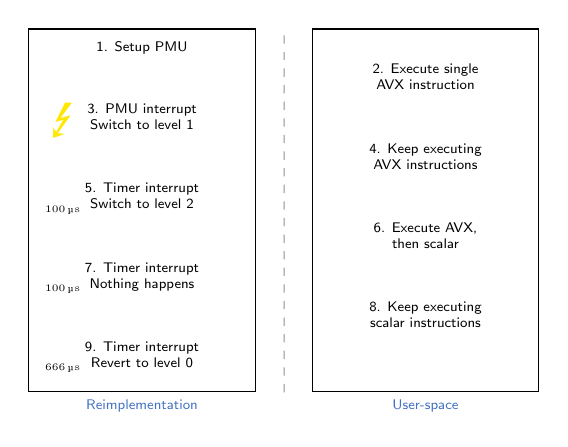
\begin{tikzpicture}[font=\scriptsize,scale=0.72, every node/.style={transform shape}]
	\sffamily
	\pgfmathsetmacro{\componentrectwidth}{4}
	\pgfmathsetmacro{\componentrectheight}{6.4}
	\pgfmathsetmacro{\separatordist}{0.5}
	\pgfmathsetmacro{\arrowoverlength}{0.25}
	\pgfmathsetmacro{\arrowlength}{2*(\arrowoverlength + \separatordist)}
	\pgfmathsetmacro{\halfcomponentrectwidth}{\componentrectwidth*0.5}
	\pgfmathsetmacro{\quartercomponentrectwidth}{\componentrectwidth*0.25}
	
	% kernel
	\draw (0cm,0cm) rectangle ++(\componentrectwidth cm,\componentrectheight) [ref=kernel-rect];
	\node[color=kitblue] at ([yshift=-0.25 cm] kernel-rect south) {Reimplementation};
	
	% separator
	\draw[dashed, color=kitdarkgrey] ([xshift=\separatordist cm] kernel-rect south east) -- ([xshift=\separatordist cm] kernel-rect north east) [ref=separator];
	
	% user-space
	\draw ([xshift=2*\separatordist cm + \componentrectwidth cm] 0, 0) rectangle ++(\componentrectwidth,\componentrectheight) [ref=user-rect];
	\node[color=kitblue] at ([yshift=-0.25 cm] user-rect south) {User-space};
	
	% steps
	\node[align=center, anchor=north] at ([yshift=-0.1cm] kernel-rect north) {1. Setup PMU};
	
	\node[align=center, anchor=north] at ([yshift=-0.5cm] user-rect north) {2. Execute single \\ AVX instruction};
	
	\node[align=center, anchor=north, color=kityellow] at ([yshift=-1.2cm, xshift=-1.4cm] kernel-rect north) {\Huge\Lightning};
	\node[align=center, anchor=north] at ([yshift=-1.2cm] kernel-rect north) {3. PMU interrupt \\ Switch to level 1};
	
	\node[align=center, anchor=north] at ([yshift=-1.9cm] user-rect north) {4. Keep executing \\ AVX instructions};
	
	\node[align=center, anchor=north, color=kitdarkgrey] at ([yshift=-2.55cm, xshift=-1.4cm] kernel-rect north) {\small\Interval};
	\node[align=center, anchor=north] at ([yshift=-3cm, xshift=-1.4cm] kernel-rect north) {\tiny\SI{100}{\micro\second}};
	\node[align=center, anchor=north] at ([yshift=-2.6cm] kernel-rect north) {5. Timer interrupt \\ Switch to level 2};
	
	\node[align=center, anchor=north] at ([yshift=-3.3cm] user-rect north) {6. Execute AVX, \\ then scalar};
	
	\node[align=center, anchor=north, color=kitdarkgrey] at ([yshift=-3.95cm, xshift=-1.4cm] kernel-rect north) {\small\Interval};
	\node[align=center, anchor=north] at ([yshift=-4.4cm, xshift=-1.4cm] kernel-rect north) {\tiny\SI{100}{\micro\second}};
	\node[align=center, anchor=north] at ([yshift=-4cm] kernel-rect north) {7. Timer interrupt \\ Nothing happens};
	
	\node[align=center, anchor=north] at ([yshift=-4.7cm] user-rect north) {8. Keep executing \\ scalar instructions};
	
	\node[align=center, anchor=north, color=kitdarkgrey] at ([yshift=-5.35cm, xshift=-1.4cm] kernel-rect north) {\small\Interval};
	\node[align=center, anchor=north] at ([yshift=-5.8cm, xshift=-1.4cm] kernel-rect north) {\tiny\SI{666}{\micro\second}};
	\node[align=center, anchor=north] at ([yshift=-5.4cm] kernel-rect north) {9. Timer interrupt \\ Revert to level 0};
	\end{tikzpicture}
\end{figure}
\end{frame}

\begin{frame}[t]{Oracle Mechanism}
	\begin{itemize}
		\item Want to find theoretical limit for optimized algorithms
		\begin{itemize}
			\item[$\Rightarrow$] implement oracle mechanism
		\end{itemize}
		\item System call API to tell reimplementation when to switch frequency levels
		\item Synthetic workload with scalar and vector phases
		\begin{itemize}
			\item[$\Rightarrow$] scalar phases of about \SI[quotient-mode=fraction]{2/3}{\milli\second} expose worst case
			\begin{itemize}
				\item hardware's worst case is best case for oracle
			\end{itemize}
		\end{itemize}
	\end{itemize}
\end{frame}
\chapter{Evaluation}
\label{sec:evaluation}

We have presented the design of \textsc{avxfreq}, a software-based reimplementation of a partial model of Intel's \gls{AVX} reclocking algorithm, in the previous chapter. Further, we have described how \textsc{avxfreq} can be leveraged to allow user-space programs to choose the applied turbo license levels themselves. In this chapter, we will evaluate these implementations: in the case of \textsc{avxfreq}, we will present modifications to \textsc{avxfreq} itself as well as the analysis framework previously presented in \Cref{sec:analysis} that allow us to use the latter in order to compare \textsc{avxfreq}'s behavior to Intel's hardware implementation and the simplified algorithm we wanted to reflect. For the user-space-driven decisions we will describe the design of a simple program that simulates heterogeneous workloads with both scalar and \gls{AVX} instructions. Finally, we will present the results obtained from executing these tests.

\section{Design}
\label{sec:evaluation:design}

% TODO text here

\subsection{\textsc{avxfreq}}
\label{sec:evaluation:design:avxfreq}

To be able to evaluate the quality of \textsc{avxfreq}'s implementation and to measure how good it reflects the hardware's reclocking behavior, it seems a good idea to make use of the analysis framework from \Cref{sec:analysis} -- in the best case, running it with \textsc{avxfreq} should deliver similar results to what is seen with hardware reclocking. However, our framework relies on using the processor's \gls{PMU} (as described in \Cref{sec:analysis:design:pmu}), just like \textsc{avxfreq} does, and, due to the limited amount of available performance counters they may not use the \gls{PMU} concurrently. Further, hardware-side performance events that count cycles a processor's core spends in a specific turbo license level do not make sense anymore when \textsc{avxfreq} is enabled as the license levels are now emulated by software.

To circumvent these obstacles, we adapted \textsc{avxfreq} and our analysis framework to work together to emulate the most important performance events in software: the idea is that \textsc{avxfreq} already uses some of the performance events that the analysis system would need anyway and that it is perfectly capable of counting cycles spent in different states. Therefore, we let \textsc{avxfreq} do the bookkeeping and provide our framework's kernel component with software-generated events instead of interrupts in a manner that is completely transparent to the user-space part.

\textsc{avxfreq} in itself only needs one performance counter to count retired \SI{512}{\bit} floating-point double-precision packed vector operations and, apart from that, also makes use of a fixed counter to count core cycles. Thus, we need to provide these to the analysis framework's kernel module -- other counters may be managed by the module itself. For this purpose, \textsc{avxfreq} keeps raw counters in software that are updated using the values provided by the \gls{PMU} whenever any event triggers \textsc{avxfreq} code to be run. To enable interaction between the analysis framework's kernel module and \textsc{avxfreq}, we defined and implemented the following kernel-internal interface:

\begin{itemize}
	\item \mintinline{c}{bool avxfreq_is_enabled(void)} \\
		Returns \mintinline{c}{true} if \textsc{avxfreq} was enabled during system boot, \mintinline{c}{false} otherwise. If \textsc{avxfreq} is not enabled, there is no reason for the analysis framework to do anything differently.
	\item \mintinline{c}{avxfreq_counters *avxfreq_get_counters(int cpu)} \\
		\mintinline{c}{avxfreq_counters} is a C language \mintinline{c}{struct} that contains the raw counters for the values defined above. One instance is defined for every core in the system. Given a core number, this method returns a pointer to the instance for the respective core.
	\item \mintinline{c}{void avxfreq_reset_cycle_counter(void)} \\
		This method resets the current core's cycle fixed counter. % TODO why the fuck do we need this
	\item \begin{minted}[autogobble]{c}
			void avxfreq_set_license_transition_listener
			     (avxfreq_license_transition_listener listener)
		\end{minted}
		\vspace{-0.45cm} % TODO what's the correct value here?
		Using this method, the analysis kernel module can hook into \textsc{avxfreq} and receive notifications whenever the applied virtual license level changes. The argument provided is a pointer to a function that takes two arguments: the previous virtual license level and the new one.
\end{itemize}

Using this interface, we modify our kernel component as follows: when loaded, it calls \texttt{avxfreq\_is\_enabled()} to check whether \textsc{avxfreq} is active. If so, it will not reconfigure the \gls{APIC} to take over handling of \gls{PMU} interrupts, but rather call \texttt{avxfreq\_set\_license\_transition\_listener()} to receive updates from \textsc{avxfreq} about license level switches and \texttt{avxfreq\_get\_counters()} once for every \gls{CPU} core in the system to locally store pointers to all counters provided by \textsc{avxfreq}. In addition to the raw counters, we added a local structure that contains derived counters, e.g., \textsc{avxfreq} only counts core cycles since they were last reset, but we also need to be able to distinguish cycles spent in the different license levels.

Whenever the module needs to write to \gls{PMU} \glspl{MSR} after being instructed to do so by the user-space component (e.g., during the \texttt{SETUP ioctl()}), it stores updated performance counter configurations in an array, so that it can later map them to software counters from \textsc{avxfreq}. Direct writes to performance counters are remapped to the corresponding software counters, unless there is no software counter available for them -- in this case, they are routed to the \glspl{MSR} just like when \textsc{avxfreq} is disabled. Similar action is taken when trying to read performance counters. This way, \gls{PMU} configuration remains fully transparent to user-space and hardware counters are automatically remapped to software counters when required without need for further intervention.

Interrupt handling is, as previously mentioned, disabled in case \textsc{avxfreq} is enabled. Instead, when the \texttt{avxfreq\_license\_transition\_listener} is called, it will update all local software counters with the values currently set in \textsc{avxfreq}'s counters and trigger the interrupt handler if the license level transition reflects one for which user-space requested an interrupt. Again, using this mechanism, we substitute hardware interrupts with software-based events in a manner that is transparent to user-space.

The interrupt handler itself (which now does not necessarily handle \emph{interrupts}) only needs a very small modification to work in this scenario: it must not reset the interrupt state in hardware, both for the \gls{PMU} and the \gls{APIC}. Apart from that, all interrupt actions we defined in \Cref{sec:analysis:design:kernel} work the same way as before.

As shown, these modifications allow us to fully employ our analysis framework with all its features and without drawbacks in combination with \textsc{avxfreq} enabled.

\section{Results}
\label{sec:evaluation:results}

\section{Future Work}
\begin{frame}[t]{Future Work}
	\begin{itemize}
		\item Implement alternative reclocking algorithms
		\begin{itemize}
			\item Take ideas from power management
		\end{itemize}
		\item More analysis
		\begin{itemize}
			\item Other processors (Haswell, Icelake)
			\item SMT
			\item Instruction mixtures
		\end{itemize}
		\item Reverse engineer AVX frequency offset configuration
	\end{itemize}
\end{frame}
\section{Conclusion}
\begin{frame}[t]{Conclusion}
	\begin{itemize}
		\item Performance of workloads with scalar and vector phases suffers from AVX reclocking
		\item We want to find improvements to the reclocking behavior
		\item Intel's claims about the algorithm are not accurate
		\item Improvements for heterogeneous workloads are theoretically possible
		\begin{itemize}
			\item up to \SI{15}{\percent} performance increase
		\end{itemize}
		\item Possibilities for software reimplementation are limited
		\begin{itemize}
			\item Still a potentially promising approach
			\item Improvements likely possible
		\end{itemize}
	\end{itemize}
\end{frame}

\end{document}